\chapter{Предложенный алгоритм}

Для решения нашей задачи нужно для начала разобраться с двумя вопросами:

\begin{enumerate}
  \item Как оценивать плотность итогового подграфа?
  \item Что такое <<большинство вершин-запросов>>?
\end{enumerate}

Для сравнения подгафов, полученных разными алгоритмами мы будем использовать реберную плотность и размер итогового подграфа: $density(G) = \frac{2 \cdot |E(G)|}{|V(G)| \cdot (|V(G)| - 1)}$, $size(G) = |V(G)|$. Действительно, если ребер в полученном подграфе достаточно много, можно считать, что он плотный. Однако также хочется, чтобы при этом он имел как можно меньший размер. Что же такое <<большинство вершин-запросов>> в подграфе-ответе мы обсудим чуть позже.

\section{Описание идеи алгоритма}

Так как алгоритмов, решающих именно нашу задачу, слишком мало, у нас есть два подхода к решению поставленной задачи~--- придумать полностью новый алгоритм или усовершенствовать один из существующих, требующих наличие всех вершин-запросов в ответе. Далее для описания задачи поиска сообщества, содержащего все выделенные вершины-запросы мы будем использовать сокращение \textit{CSP}, а для нахождения сообщества, содержащего большинство вершин-запросов~--- \textit{NCSP}.

Полностью новым алгоритмом будет, например, следующий: перебрать множество вершин, которое по нашему мнению является шумом, найти подграф, содержащий все остальные вершины одним из существующих алгоритмов, требующих наличие всех вершин-запросов, а затем обновить ответ. Это решение имеет место быть и даже будет выдавать наиболее оптимальный ответ, однако понятно, что это слишком долго~--- перебор множества игнорируемых вершин будет иметь экспоненциальную от их количества асимптотику, которая затем умножается еще и на асимптотику выбранного алгоритма, ищущего CSP для оставшихся вершин. Поэтому мы не будем использовать этот метод, а попытаемся предложить что-нибудь другое.

Более простым путем будет усовершенствование идеи одного из последних алгоритмов, решающих CSP. Действительно~--- идея (что именно оптимизировать) уже проверена и показала неплохие результаты, и если применить другие эвристики, которые позволят учитывать постановку нашей задачи, может получиться неплохой результат. Так мы и сделаем: возьмем алгоритм Barbieri et al. \cite{Barbieri15} и попробуем его расширить на нашу задачу. Статьи Bogdanov et al. \cite{Bogdanov13} и Cui et al. \cite{Cui14} показали, что максимизация минимальной степени вершины является эффективным способом нахождения оптимального сообщества, поэтому наша идея имеет место быть. 

Идея алгоритма Barbieri et al. \cite{Barbieri15} заключается в нахождении в графе $G$ \textit{k-core} с максимальным $k$, а также минимального размера, содержащим все вершины из $Q$. В статье авторы показывают, что это NP-полная задача, а следовательно для ее решения нужны эвристики. Это не является плохой стороной, потому что на данный момент не существует алгоритмов, в которых задача, оптимизируемая для поиска оптимального сообщества, является решаемой за полиномиальное время, а сами алгоритмы показывают хорошие результаты. Так, например, Sozio et al. \cite{Sozio10} ищут \textit{k-core} с максимальным $k$, не обращая внимание на минимальность его размера. Эта задача оказывается решаемой за линейное время от количества ребер в графе, однако, этот алгоритм выдает слишком большие подграфы. Введение же параметра $size$, ограничивающего размер итогового подграфа сразу делает задачу NP-полной, что авторы и показывают в статье.

Возвращаясь к статье Barbieri et al. \cite{Barbieri15}, отметим главную идею их алгоритма. Алгоритм опирается на следующее утверждение: если взять ядерную декомпозицию $C = \{C_k\}_{k=1}^{k=k^*}$ графа $G$, а затем найти такое максимальное $k'$, что все вершины из запроса $Q$ лежат в одной и той же компоненте $H^* \in C_{k'}$, то все ответы на CSP находятся в этой компоненте $H^*$. Более формально: $k' = \max\{k | \exists H_i\mbox{~--- компонента связности } C_{k'}\mbox{, т.ч. } \forall v \in Q: v \in H_i\}$. Найденный \textit{k-core} мы будем обозначать $C_Q^*$, а компоненту, содержащую все вершины из $Q$~--- $H^*$. Стоит отметить две вещи: во-первых, это утверждение позволяет сразу же перейти нам к более маленькому подграфу без потери решений, а во-вторых, это утверждение верно и для нашей задачи: раз $H^*$ содержит все оптимальные подграфы, содержащие все вершины из $Q$, то и подграфы, содержащие большинство вершин из $Q$, он тоже содержит (возможно, в нашем ответе \textit{k-core} будет более высокого порядка, однако, ничто не мешает нам начать оптимизировать ответ с $H^*$).

Опишем итоговую идею нашего алгоритма: по данному графу $G$ и запросу $Q$, мы будем выделять \textit{k-core} $C_Q^*$ и его компоненту связности $H^*$, содержащую все оптимальные ответы на NCSP. $H^*$ сам вполне подходит под ответ, потому что содержит все вершины из $Q$, однако его размер в среднем получается довольно большим, что нас не устраивает (а также этот подграф содержит все вершины-запросы, а следовательно содержит и шум). Поэтому после нахождения $H^*$ мы предложим эвристики, позволяющие уменьшить его размер, сохраняющие условие на минимальную степень вершины, а следовательно и не ухуджающие плотность ответа.

\section{Описание алгоритма}

В этом разделе мы опишем сам алгоритм. Фактически, сейчас мы можем разделить алгоритм на две фазы:

\begin{enumerate}
  \item Выделение по данному запросу $Q$ \textit{k-core} $C_Q^*$ и его компоненты $H^*$;
  \item Уменьшение размера $H^*$ с сохранением свойств на минимальную степень вершины.
\end{enumerate}

На самом деле, в дальнейшем мы разделим вторую фазу еще на несколько, однако об этом будет написано позднее. Сейчас мы попробуем разобраться с каждой фазой по отдельности.

\subsection{Фаза 1. Нахождение $C_Q^*$ и $H^*$}

Фазу выделения $C_Q^*$ и $H^*$ мы позаимствуем из статьи Barbieri et al. \cite{Barbieri15}, как и их идею о минимизации \textit{k-core}. Несложно заметить, что ядерная декомпозиция не зависит от запроса, поэтому нет смысла строить ее каждый раз, так как это занимает достаточно много времени. Однако и сохранить ее в оперативной памяти перед всеми запросами мы тоже не можем, потому что ее размер слишком велик для этого. Поэтому мы сделаем предподсчет, который один раз построит ядерную декомпозицию и сохранит ее в сжатом виде на диск. Это будет так называемый индекс, который позволит по запросу $Q$ намного быстрее, чем раньше, находить $C_Q^*$ и $H^*$ из уже построенной ядерной декомпозиции.

В нашем индексе ядерной декомпозиции $C = \{C_k\}_{k = 1}^{k = k^*}$ мы будем хранить следующую информацию:

\begin{enumerate}
  \item Ядерные индексы всех вершин $c(v) = \max\{k \in [0..k^*] | v \in C_k \}$;
  \item Для каждого \textit{k-core} $C_k$ будем хранить набор его компонент $C_k = \{H_i\}$.
\end{enumerate}

Описание вышесказанного иллюстрирует рисунок~\ref{index-construct}:

\begin{figure}[!h]
\caption{Построение индекса}\label{index-construct}
\centering
  \begin{center}
    \makebox[\textwidth]{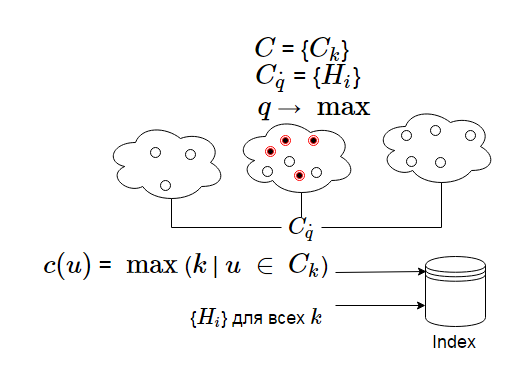
\includegraphics[scale=0.8]{pictures/index.png}}
  \end{center}
\end{figure}
\FloatBarrier

Стоит также сделать небольшое замечание, что некоторые соседние \textit{k-core} равны: $C_k = C_{k + 1}$. Нет смысла хранить их два раза, поэтому все повторяющиеся соседние \textit{k-core} мы будем хранить только один раз. Сейчас это кажется не очень хорошей оптимизацией, однако на реальных данных количество различных \textit{k-core} на несколько порядков меньше общего их количества, поэтому эта оптимизация имеет смысл. При описании дальнейших действий мы будем использовать переменную $h$~--- она означает количество различных \textit{k-core} в нашей ядерной декомпозиции, то есть количество \textit{k-core}, которые мы будем хранить в индексе.

Хранить ядерные индексы и набор компонент мы будем в соответствующих структурах данных (хеш-таблицах), позволяющих получать доступ к $c(v)$, набору всех компонент фиксированного \textit{k-core}, а также к компоненте фиксированного \textit{k-core}, в которой находится выбранная вершина $v$, за $O(1)$.

Однако мы до сих пор не сказали, как построить этот индекс. Строить его мы будем довольно просто: сначала построим набор компонент для $C_{k^*}$, а все остальные \textit{k-core} будем строить следующим образом: если уже построены \textit{k-core} порядков $k^*, k^*-1, \ldots, k$, то для построения \textit{$(k - 1)$-core} мы по одной добавим все вершины из $C_{k - 1} \setminus C_k$  и ребра, инцидентные им (благодаря свойству, что $C_{k - 1} \supseteq C_k$, этого достаточно), а затем обновим компоненты связности, которые благодаря новым вершинам могут объединиться в новые, более большие компоненты.

Эта фаза занимает $O(h \cdot |V(G)| + |E(G)|)$ времени, или же по-простому $O(hn + m)$, где $h$, напомним, количество различных \textit{k-core} в $G$. Однако эту асимптотику мы не будем учитывать в итоговом подсчете, потому что для каждого графа эта операция производится один раз, а затем построенный индекс используется для нахождения $C_Q^*$ и $H^*$.

Так как же найти $C_Q^*$ и $H^*$ по построенному индексу? На самом деле, очень просто. Так как $C_1 \supseteq C_2 \ldots \supseteq C_{k^*}$, то для нахождения \textit{k-core} наибольшего порядка, содержащего все вершины $Q$ в одной своей компоненте, мы можем использовать двоичный поиск по порядку \textit{k-core}. Чтобы проверить для фиксированного $C_k$, правда ли, что все вершины из $Q$ находятся в одной его компоненте, мы достанем из индекса информацию о компоненте для каждой вершины-запроса (напомним, что эта операция выполняется за $O(1)$), а затем проверим, что все эти числа получились одинаковые. Таким образом, проверка шага двоичного поиска происходит за $O(|Q|)$.

Суммируя все вышесказанное, получаем, что шаг нахождения $C_Q^*$ и $H^*$ выполняется за $O(|Q| \cdot \log(h))$.

\subsection{Фаза 2. Уменьшение размера $H^*$}

После выделения из графа $G$ \textit{k-core} $C_Q^*$ и его компоненты связности $H^*$, содержащей все вершины из $Q$, как мы уже отмечали, можно заметить, что $H^*$~--- ответ на нашу задачу, ведь степени всех его вершин хотя бы $k$ (то есть это \textit{k-core}), причем это $k$~--- максимально возможное (по построению $H^*$). Однако, не соблюдается одно оставшееся условие в постановке задачи~--- этот \textit{k-core} не минимального размера. Это мы и попытаемся исправить в этой и $3$-й фазах. Именно в этой фазе мы ставим перед собой следующую задачу: сейчас $H^*$ содержит все вершины-запросы, однако мы знаем, что среди них может быть шум. Задача этой фазы~--- выделить подграф, не содержащий шумовые вершины.

Напомним, что задача нахождения минимального по размеру \textit{k-core}~--- NP-полная. Какие эвристики мы можем применить? Первая мысль, которая приходит в голову~--- удалять слабо связанные вершины или подграфы из $H^*$, тем самым уменьшая его размер. Однако, так как степени всех вершин хотя бы $k$, сложно понять, какие вершины слабо связаны и удаление каких подграфов не нарушит свойство на степени вершины, то есть оставит подграф плотным. 

Нами был выбран обратный подход~--- добавление вершин. Будем строить итоговый подграф $H_{min}$ следующим образом: возьмем все вершины-запросы $Q$, удалим остальные вершины и ребра. Затем будем добавлять по одной вершине с некоторым приоритетом, тем самым постепенно увеличивая наш текущий подграф $H_{min}$. В каждый момент времени, когда текущий граф будет удовлетворять ответу на нашу задачу (то есть что компонента $H_{min}$, содержащая наибольшее количество вершин-запросов, содержит <<большинство вершин из $Q$>>, а также она довольно <<плотная>>), мы будем обновлять ответ. Понятно, что процесс не бесконечный~--- количество вершин в текущем ответе постоянно увеличивается, но подграф больше, чем $H^*$, мы не получим. Однако перед нами встает три глобальных вопроса:

\begin{enumerate}
  \item Какой выбрать приоритет для добавления вершин?
  \item Когда именно обновлять ответ (что такое <<большинство вершин из $Q$>>, что такое <<компонента довольно плотная>>)?
  \item Когда останавливать добавление вершин?
\end{enumerate}

\textbf{a. Какой приоритет использовать для добавления очередной вершины?}

Вариантов приоритета может быть множество. Однако давайте подумаем, что для нас важно в первую очередь. Во-первых, мы хотим, чтобы вершины, образующие сообщество (то есть набор вершин-запросов без шума), как можно быстрее объединились в связную компоненту и начали наращивать ее плотность. Для этого первым приоритетом сделаем количество компонент, которое объединяет вершина при добавлении. То есть, $p_1(v) = |A'| - |A|$, где $A$~--- множество компонент до добавления, а $A'$~--- после. Однако довольно часто при добавлении очередной вершины количество компонент остается неизменным. Что делать в этом случае? Так как для нас также важны степени вершин в итоговом подграфе, давайте акцентируем на этом внимание. При добавлении вершины $v$ степени вершин ее соседей, уже содержащихся в текущем подграфе, увеличиваются на $1$. Нам бы хотелось максимизировать это количество. Однако, нужно также учесть только что добавленную вершину и ее степень. Сделаем вторым приоритетом $p_2(v) = |N_{H_{min}}(v) \cap \{v \in V(H_{min}) | deg(v) < \mu(H^*)\}| - \max(0, \mu(H^*) - |N_{H_{min}}(v)|)$, где $N_{H_{min}}(v)$~--- множество вершин из $H_{min}$, соединенных с $v$ ребром. Другими словами, мы учитываем со знаком плюс количество вершин-соседей вершины $v$ из $H_{min}$, степень вершин которых еще меньше требуемой $\mu(H^*)$, а со знаком минус учитываем количество ребер, которое не хватает только что добавленной вершине до требуемой степени $\mu(H^*)$.

\textbf{b. Что же такое <<большинство вершин из $Q$>>, что значит <<компонента довольно плотная>>?}

Мы будем говорить, что подграф $H \subset G$ содержит большинство вершин из $Q$, если количество вершин-запросов в нем хотя бы $\alpha(|Q|) \cdot |Q|$. $\alpha(|Q|) \in (0, 1]$ или просто $\alpha$~--- некий коэффициент, зависящий от количества вершин-запросов. Какие же значения должно принимать $\alpha$? С одной стороны, мы хотим, чтобы <<большинство вершин>> было действительно большинством, поэтому мы будем считать, что шума в запросе меньше $\frac{|Q|}{2}$ (то есть $\alpha \ge 0.5$). С другой стороны, даже $\frac{|Q|}{2}$ вершин почти всегда слишком много для шума.  

Нас также интересует, что значит <<компонента довольно плотная>>. Будем говорить, что компонента довольно плотная, если в ней достаточно много ребер (то есть и плотность достаточно большая). Для выбора границы количества ребер было попробовано несколько функций, оптимальной оказалось следующая: $|E(H_{min})| \ge (V(H_{min}) - |Q|) \cdot \mu(H^*) + \beta(|Q|) \cdot |Q|)$, то есть у всех вершин-запросов степень вершин берется равной $\beta$ (еще один параметр), а у остальных она должна быть хотя бы $\mu(H^*)$ (на самом деле, если в запросе есть шум, степень вершины должна быть больше, однако, если шума нет, это неправда). 

На самом деле, условие на плотность компоненты можно не учитывать, а просто проверять, что текущий подграф содержит <<большинство вершин из $Q$>>~--- ведь в зависимости от этих условий мы только решаем, обновлять ли ответ. Однако, условие на плотность компоненты было добавлено с целью уменьшения количества обновлений ответа и уменьшения времени работы алгоритма.

Для выбора оптимальных значений параметров $\alpha$ и $\beta$ по фиксированному $|Q|$ было решено провести исследование. Исследование проводилось на тех же экспериментах, что и сравнение различных алгоритмов (об этом подробнее в главе $3$). Результаты исследований приведены в таблице ниже ($k$~--- порядок \textit{k-core}, то есть $k = \mu(H^*)$).

\begin{table}[!h]
\centering
\caption{Оптимальные значения параметров $\alpha$ и $\beta$ для различных $|Q|$}\label{parameters-research}
  \begin{tabular}{| l | l | p{1cm} |}
  \hline
  $|Q|$ & $\alpha$ & $\beta$ \\\hline
  2   & 1      & 1        \\\hline
  3   & 2 / 3  & 1        \\\hline
  4   & 1 / 2  & 1        \\\hline
  5   & 3 / 5  & 2        \\\hline
  6   & 2 / 3  & 2        \\\hline
  7   & 4 / 7  & 3        \\\hline
  8   & 3 / 4  & 3        \\\hline
  > 8 & 7 / 10 & 4        \\\hline
  \end{tabular}
\end{table}
\FloatBarrier

\textbf{c. Когда останавливать алгоритм добавления?}

Понятно, что остановить его можно, когда мы например добавили все вершины из $H^*$. Однако, так как размер $H^*$ может быть достаточно большим, это не самое оптимальное решение~--- после того, как наш подграф станет связным, он уже будет содержать все вершины-запросы, а следовательно и весь шум, в то время как наша задача как раз от него избавится. Поэтому будем останавливать алгоритм, когда все компоненты объединились в одну, то есть текущий подграф стал связным.

\begin{figure}[!h]
\caption{Пример работы фазы $2$}\label{phase2-example}
\centering
  \begin{center}
    \makebox[\textwidth]{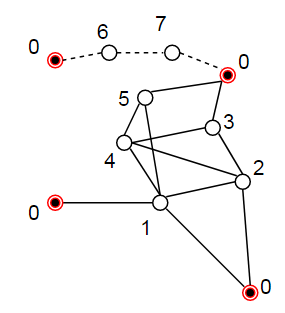
\includegraphics[scale=1.2]{pictures/phase2.png}}
  \end{center}
\end{figure}

Например, пусть $H^*$ выглядит так, как на рисунке~\ref{phase2-example} (таким он взят для упрощения и более простого объяснения и понимания написанного выше текста). Вершины-запросы в нем отмечены красным, их мы возьмем первыми (шаг $0$). Затем будем добавлять вершины по одной, в порядке, как показано на рисунке: сначала добавляем вершину $1$, потому что она объединяет две компоненты, затем $2$, потому что у нее максимальный второй приоритет, и т.д. Закончим мы, когда $H_{min}$ станет связным, то есть в данном случае, когда мы добавим все его ребра. Однако, оптимальным ответом будет подграф, не содержащий пунктирные ребра, потому что он более плотным. И, как мы видим, действительно, не добавленная вершина~--- явный шум, добавлять ее в ответ не стоит.

\subsection{Фаза 3. Восстановление условия на степень вершин}

После того, как мы выполнили фазу $2$, мы нашли подграф, который будем обозначать $H_{min}^*$. Этот подграф можно было бы вернуть как ответ, но, как мы только что видели на рисунке~\ref{phase2-example}, вполне может оказаться, что $H_{min}^*$ далек от идеального ответа. Почему? Ведь мы добавляли вершины по одной с, как нам казалось, оптимальным приоритетом. На самом деле, так как в первую очередь мы стремимся добавлять вершины, которые лучше всего объединяют наши текущие компоненты, и следим за степенями вершины только во вторую очередь (при этом фактически мы только пытаемся удовлетворить условие на степени вершин, но это не факт, что точно получится), ответ может получиться неоптимальным. Поэтому с $H_{min}^*$ надо что-то сделать, чтобы удовлетворить условие на степени вершин.

Сейчас может показаться, что фаза $2$ была вообще лишней, ведь мы из \textit{k-core}, который достаточно плотно связан благодаря условиям на степени вершин, сделали что-то непонятное, казалось бы только хуже. Это не так, потому что во-первых исходный $H^*$ содержал все вершины-запросы, в том числе шум, а подграф-ответ может быть намного плотнее. Во-вторых, это только временно, сейчас мы применим несколько эвристик и подграф станет плотным \textit{k-core} б\'{о}льшего порядка.

Для начала давайте удалим слабо связанные вершины. Так как теперь наш подграф не \textit{k-core}, мы можем предложить логичные условия для этого. Вспомним про наш введенный параметр $\beta$, который отвечал за минимальные степени вершин-запросов. Давайте удалим все вершины-запросы, имеющие степень меньше $\beta$, то есть не подходящие под наше описание (такие вершины могли остаться, потому что мы смотрели только на общее количество ребер подграфа, а не на степени вершин).

После удаления слабо связанных вершин-запросов выполним еще раз фазу $1$ уже на оставшихся запросах. На самом деле, всю фазу нам выполнять не нужно, от этой фазы нам нужно только новое значение $k^{opt}$~--- наибольший порядок \textit{k-core}, в котором все оставшиеся вершины-запросы лежат в одной компоненте связности.

Теперь мы сделаем главный шаг этой завершающей фазы. Его идея заключается в следующем: возьмем все оставшиеся выделенные вершины и найдем минимальное количество не выделенных, которые их соединяют. То есть, взяв множество оставшихся выделенных вершин $Q' \subseteq Q$, мы хотим найти такое множество вершин $V_{opt} \subseteq V(H_{min}^*) \setminus Q'$ минимального размера, что $G[V_{opt} \cup Q']$~--- связен (напомним, $G[V]$~--- подграф, порожденный множеством вершин $V$). Это даст нам <<каркас>> подграфа $H_{min}^*$, который мы сможем после этого нарастить, почти как в фазе $2$.

То, что мы описали выше~--- ничто иное как задача Штейнера. Оригинальная задача Штейнера звучит так: по данному взвешенному графу $G$ и выделенным в нем множеству вершин $Q$, найти минимальное остовное дерево на этих вершинах. Занимательный факт состоит в том, что если $|Q| = 2$, то задача сводится к кратчайшему пути в графе, если $|Q| = |V(G)|$, то задачу сводится к построению минимального остовного дерева в графе, но если оба этих условия не выполняются, задача становится NP-полной. Можно отметить, что в нашей задаче граф не взвешенный, однако задача Штейнера остается NP-полной даже в случае, когда все веса в графе одинаковые. Задача Штейнера была давно изучена, и в статье Kou et al. \cite{Kou81} был представлен оптимальный алгоритм ее решения с аппрокцимацией $2 - \frac{2}{|Q|}$ и доказательством того, что за полиномиальное время задачу Штейнера нельзя решить лучше. Мы воспользуемся решением из этой статьи и применим его к нашей задаче.

Найдя искомый <<каркас>>, применим к нему слегка измененную фазу $2$. Во-первых, каркас уже связен и нам не нужен приоритет на количество объединенных компонент. Во-вторых, хотелось бы усовершенствовать эту фазу, чтобы строго гарантировать плотность итогового подграфа. Поэтому мы меняем фазу $2$ следующим образом:

\begin{enumerate}
  \item Добавлять вершины будем только по второму приоритету (на самом деле, можно оставить и первый, просто он не будет нести никакого смысла);
  \item Останавливаться будем, когда минимальная степень вершины станет хотя бы $k^{opt}$, ведь мы точно знаем, что на оставшихся вершинах-запросах можно построить \textit{$k^{opt}$-core};
  \item Мы не будем по ходу добавления вершин обновлять ответ, ответом будет просто финальный подграф.
\end{enumerate}

Изменив фазу $2$ описанным выше образом, мы запускаем ее на $H_{min}^*$ с удаленными слабо связанными вершинами-запросами и получаем итоговый ответ на задачу.

\begin{figure}[!h]
\caption{Пример работы фазы $3$}\label{phase3-example}
\centering
  \begin{center}
    \makebox[\textwidth]{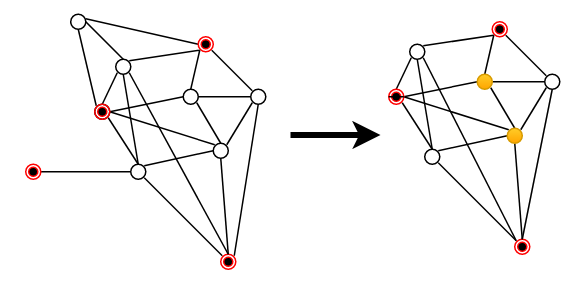
\includegraphics[scale=1.0]{pictures/phase3.png}}
  \end{center}
\end{figure}

Работа этой фазы представлена на рисунке~\ref{phase3-example}, где исходный подграф $H_{min}^*$ (который до фазы $2$ являлся \textit{3-core})находится слева, а полученный после обработки~--- справа. Сначала мы удалили явно слабо связанную вершину-запрос, а затем выделили с помощью задачи Штейнера две желтые вершины, связывающие $3$ оставшихся запроса и образующих тем самым <<каркас>> из $5$ вершин. После этого мы запускаем измененную фазу $2$ и получаем ответ, представленный справа на рисунке. Как видно, он получился меньше и плотнее, а также является \textit{4-core} вместо \textit{3-core}.

\section{Теоретическая оценка качества}

Сложно оценивать качество алгоритма без проверки на практических данных. Однако в этом разделе мы отметим несколько явных преимуществ по сравнению с имеющимися алгоритмами.

\begin{itemize}
  \item Наш алгоритм учитывает шум в запросе, если он есть и его меньше половины, а также требует наличие всех вершин в запросе, если явного шума нет;
  \item Наш алгоритм должен работать не хуже Barbieri et al. \cite{Barbieri15}, потому что мы в итоге находим \textit{k-core} порядка хотя бы $\mu(H^*)$. Наш алгоритм может работать хуже из-за отличающейся эвристики, однако на запросах с шумом мы должны находить \textit{k-core} с б\'{о}льшим порядком, а следовательно плотнее;
\end{itemize}

\chapterconclusion

В этой главе был подробно описан предложенный алгоритм решения поставленной задачи. Алгоритм состоял из трех фаз, последовательно оптимизирующих ответ на задачу. Несмотря на то, что задача NP-полная и невозможно предложить алгоритм, решаюший ее за полиномиальное время, наши эвристики позволяют, хоть и в теории, но судить о том, что результаты должны быть лучше, чем у существующих сейчас алгоритмов, однако подтверждение этому можно будет увидеть только после проведения практических результатов.

Также заметим, что наш алгоритм может поддерживать обратную совместимость~--- несложно будет добавить настраиваемый параметр $minSize$, который будет означать минимальное количество вершин-запросов, которое должно быть в ответе. Тогда в фазе $2$ мы не будем прекращать наращивать $H_{min}^*$, пока количество вершин-запросов в нем не станет хотя бы $minSize$, а в фазе $3$ не будем удалять слабо связанные вершины-запросы. Тем самым, фактически, мы можем все еще решать CSP, а не NCSP, если это потребуется.
